\section{New-reference protocol, service provenance and cost}
\label{sec:new_protocol}
\subsection{Persona sampling and analysis}
The acquisition manifest fixes 132 new persona profiles excluded from earlier datasets. The first twelve are pilot-only; the next thirty form the formal sample. A baseline and eleven perturbations share one numeric trip. The conditions cover delay of 8 and 45 minutes, fare multipliers of 1.25 and 2.5, access increases of 5 and 20 minutes, fare--delay and fare--access combinations, PT infeasibility, and rain intensities of 0.25 and 0.9. These input values define scenarios, not all-independent unseen intervention families. The archived training-support audit is retained alongside the state manifest.

The primary planning statistic is the persona-level signed-response minus soft-KL error, averaging three training seeds and eleven contrasts. The pilot standard deviation is 0.006306. The prespecified rule $\max\{30,\lceil(1.96s/0.01)^2\rceil\}$, with a maximum of 120, yields thirty formal personas. It is a precision planning rule, not a guarantee of interval width. Formal analysis uses 10,000 paired-persona bootstrap draws (seed 20260925), retaining the complete contrasts within persona. All other method, selector and condition comparisons are descriptive, with pointwise intervals. The pilot is never pooled with the formal sample.

\begin{figure}[pos=htbp]
\centering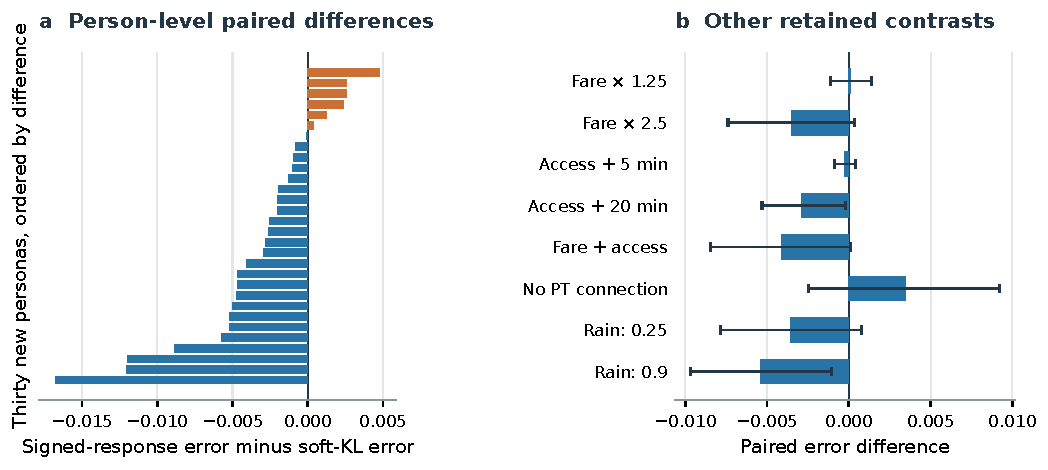
\includegraphics[width=\linewidth]{figures/revision20260925/figureA_generalization.pdf}
\caption{Additional formal-sample views under full training and KL selection. (a) All thirty persona-level primary paired differences. (b) The other eight retained contrasts, complementing the delay conditions in the main text. Whiskers are descriptive pointwise 95\% persona-bootstrap intervals. All comparisons use the same Go Flash reference and fixed trip.}
\label{fig:new_personas}
\end{figure}

Requests used OpenCode Go, model \texttt{deepseek-v4.1-flash}, temperature 0.2, an 8,192-token output budget and the provider's default reasoning setting. The requested and returned model strings agree. The pilot supplies 432 valid responses and the formal sample 1,080. Missing valid state--repeat units were reacquired after recorded connection or parsing failures without changing the prompt, state manifest or primary analysis. Acquisition attempts, completion identifiers, usage and prompt hashes are preserved in the experiment package. This campaign is distinct from the historical official Pro training and survey-reference campaigns.

\subsection{Returned service metadata}
During formal acquisition, some responses reported zero reasoning tokens and a different usage-detail structure while request settings and the returned model name stayed the same. The diagnostic was documented after observing those metadata and before examining formal method comparisons. Zero reported tokens do not prove absence of internal reasoning or a backend model change. No immutable backend fingerprint was available.

The formal sample has 976 positive-reasoning and 104 zero-reported-reasoning responses. Twenty-four personas have only the former and six have a mixture. The primary paired difference is $-0.00299$ ($[-0.00496,-0.00121]$) in the all-positive group and $-0.00405$ ($[-0.00770,-0.00117]$) in the mixed group. These post-hoc subgroups are confounded with acquisition time and persona order. They neither identify a reasoning-mode effect nor justify excluding data. The primary analysis includes all thirty personas and is conditional on the realized service mix.

\subsection{Recorded usage and retrospective valuation}
\label{sec:cost_summary}
The new pilot and formal campaign made 1,618 attempts, yielding 1,512 valid responses. Usage is available for 1,525 distinct completions, including thirteen invalid responses; 93 attempts have unknown usage. Recorded input and output total 2,206,391 and 4,355,420 tokens, respectively. Cached input is already included in input, and reasoning tokens are already included in output.

Using the Go rate card checked on 25 September 2026, with request-time peak/off-peak classification and reported cache usage, values the recorded total at US\$3.4952 of plan allowance \citep{opencode2026go}. Revaluing the same known tokens at all-peak, no-cache rates gives US\$5.8884. Neither estimate covers unknown usage or verifies an account debit. The US\$10 monthly subscription is a separate fixed expense and is not added to every request.

\begin{table}[pos=htbp]
\centering\small
\caption{Retained API usage repriced at the official DeepSeek V4 Pro rates checked on 25 September 2026. Costs are estimates in USD, not invoices.}
\label{tab:api_cost}
\setlength{\tabcolsep}{3pt}
\begin{tabularx}{\linewidth}{@{}Xrrrr@{}}
\toprule
Acquisition group & Metered calls & Input (M) & Output (M) & USD range \\
\midrule
Primary supervision archives & 8,681 & 10.050 & 32.614 & 65.83--131.66 \\
Final same-task reference & 1,440 & 2.324 & 3.255 & 7.08--14.16 \\
Earlier same-task campaign & 1,475 & 1.969 & 5.575 & 11.58--23.15 \\
Neutral-metadata pilot & 120 & 0.160 & 0.239 & 0.52--1.03 \\
Ownership pilot & 120 & 0.160 & 0.235 & 0.52--1.03 \\
Latency benchmark & 87 & 0.117 & 0.353 & 0.76--1.51 \\
Other historical development & 1,468 & 2.377 & 8.149 & 16.43--32.86 \\
Retained metered total & 13,391 & 17.157 & 50.418 & 102.71--205.42 \\
\bottomrule
\end{tabularx}
\par\smallskip\begin{minipage}{\linewidth}\footnotesize
Completion IDs are deduplicated across archives. Input costs use the recorded cache-hit/miss split; output includes reasoning tokens. The range reprices the same usage entirely at off-peak or peak rates, rather than reconstructing historical deductions. The primary archives contain the legacy, joint and corrected accessibility acquisition pools, including labels outside the final benchmark. Other development includes deprecated S8. A further 576 retained completions lack usage and are excluded from the monetary sum, as are unmetered failures; their cost is unknown. The earlier same-task campaign includes 35 responses rejected by parsing but with recorded token usage. This is neither the marginal cost of one fitted Student nor a full project invoice.
\end{minipage}
\end{table}

The historical Pro table above includes retained development runs and earlier model versions, not just acquisition for the final Student. It is a current-rate revaluation of observed usage rather than a recovered invoice. It must not be priced with the new Go Flash rates. The 27 controlled and six delay-withheld fits sum to 845.69 and 200.17 seconds of recorded fit time; these are neither end-to-end campaign wall times nor CPU-seconds. Hardware rental and electricity charges were not recorded.

For repeated matched workloads, a monetary break-even count would be $N^*=C_0/(c_L-c_S)$ when $c_L>c_S$, where $C_0$ includes acquisition, retries, training and necessary adaptation, and $c_L,c_S$ are comparable per-workload costs. Shared supply and routing work must be counted consistently. Existing measurements supply only part of this accounting. Supplementary Section~\ref{supp-sec:supp_compute} retains the inference, construction and historical metering details without asserting a measured lifecycle break-even point.
